\documentclass{article}
\usepackage{amsmath}
\usepackage{amssymb}
\usepackage{graphicx}
\usepackage{tikz}
\usetikzlibrary{shapes.geometric}

\begin{document}

\title{勾股定理的 LaTeX 公式}
\author{}
\date{}
\maketitle

\section{勾股定理的基本公式}

勾股定理(Pythagorean theorem)是几何学中的基本定理,描述了直角三角形三边之间的关系。

\subsection{标准公式}

对于直角三角形,设直角边为 $a$ 和 $b$,斜边为 $c$,则有:

\[
a^2 + b^2 = c^2
\]

\subsection{向量形式}

如果用向量表示,设 $\mathbf{a}$ 和 $\mathbf{b}$ 是正交向量,则:

\[
\|\mathbf{a}\|^2 + \|\mathbf{b}\|^2 = \|\mathbf{a} + \mathbf{b}\|^2
\]

\subsection{三角函数形式}

利用三角函数,勾股定理可以表示为:

\[
\sin^2\theta + \cos^2\theta = 1
\]

其中 $\theta$ 是直角三角形的一个锐角。

\section{几何证明图示}

\begin{figure}[h]
\centering
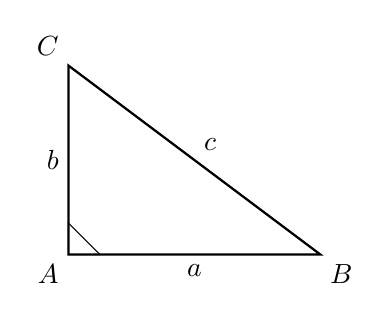
\begin{tikzpicture}[scale=0.8]
    % 绘制直角三角形
    \draw[thick] (0,0) -- (4,0) -- (0,3) -- cycle;
    
    % 标记顶点
    \node[below left] at (0,0) {$A$};
    \node[below right] at (4,0) {$B$};
    \node[above left] at (0,3) {$C$};
    
    % 标记边长
    \node[below] at (2,0) {$a$};
    \node[left] at (0,1.5) {$b$};
    \node[above right] at (2,1.5) {$c$};
    
    % 标记直角
    \draw (0,0) -- (0.5,0) -- (0,0.5) -- cycle;
\end{tikzpicture}
\caption{直角三角形 $ABC$,其中 $\angle C = 90^\circ$,$AB = c$,$BC = a$,$AC = b$}
\end{figure}

\section{相关公式推导}

\subsection{求斜边长度}

已知直角边 $a$ 和 $b$,求斜边 $c$:

\[
c = \sqrt{a^2 + b^2}
\]

\subsection{求直角边长度}

已知斜边 $c$ 和一个直角边 $a$,求另一个直角边 $b$:

\[
b = \sqrt{c^2 - a^2}
\]

\subsection{面积公式}

直角三角形的面积可以用直角边计算:

\[
S = \frac{1}{2}ab
\]

也可以用斜边和斜边上的高 $h$ 计算:

\[
S = \frac{1}{2}ch
\]

\section{勾股定理的推广}

\subsection{余弦定理}

勾股定理是余弦定理的特例。对于任意三角形:

\[
c^2 = a^2 + b^2 - 2ab\cos\gamma
\]

当 $\gamma = 90^\circ$ 时,$\cos\gamma = 0$,得到勾股定理。

\subsection{n维空间推广}

在 n 维欧几里得空间中,向量的长度满足:

\[
\| \mathbf{x} \|^2 = \sum_{i=1}^n x_i^2
\]

\section{代码示例}

\subsection{Python 实现}

\begin{verbatim}
def pythagorean_theorem(a, b):
    """计算直角三角形的斜边长度"""
    return (a**2 + b**2)**0.5

def is_right_triangle(a, b, c):
    """判断三边是否能构成直角三角形"""
    sides = sorted([a, b, c])
    return abs(sides[0]**2 + sides[1]**2 - sides[2]**2) < 1e-10
\end{verbatim}

\subsection{JavaScript 实现}

\begin{verbatim}
function pythagorean(a, b) {
    return Math.sqrt(a*a + b*b);
}

function isRightTriangle(a, b, c) {
    const sides = [a, b, c].sort((x, y) => x - y);
    return Math.abs(sides[0]**2 + sides[1]**2 - sides[2]**2) < 1e-10;
}
\end{verbatim}

\end{document}